\documentclass{article}

% if you need to pass options to natbib, use, e.g.:
 \PassOptionsToPackage{numbers, compress}{natbib}
% before loading nips_2018

% ready for submission
\usepackage{nips_2018}

% to compile a preprint version, e.g., for submission to arXiv, add
% add the [preprint] option:
% \usepackage[preprint]{nips_2018}

% to compile a camera-ready version, add the [final] option, e.g.:
% \usepackage[final]{nips_2018}

% to avoid loading the natbib package, add option nonatbib:
% \usepackage[nonatbib]{nips_2018}

\usepackage[utf8]{inputenc} % allow utf-8 input
\usepackage[T1]{fontenc}    % use 8-bit T1 fonts
\usepackage{hyperref}       % hyperlinks
\usepackage{url}            % simple URL typesetting
\usepackage{booktabs}       % professional-quality tables
\usepackage{amsfonts}       % blackboard math symbols
\usepackage{nicefrac}       % compact symbols for 1/2, etc.
\usepackage{microtype}      % microtypography

%%%%%%%%%%%%%%%%
%%%%%My Packages%%%%%
%%%%%%%%%%%%%%%%

\usepackage{amsmath, amssymb, amsthm, mathtools}

\newtheorem{theorem}{Theorem}[section]
\newtheorem{definition}{Definition}[section]

\usepackage{enumerate,xcolor}
\usepackage{tikz,hyperref}
\usetikzlibrary{spy,calc,patterns,arrows,decorations.pathmorphing,backgrounds,positioning,fit,petri,mindmap,trees,intersections}
\usepackage{algorithm}
\usepackage{algorithmic}
\usepackage{bm}

\def\CC{{C\nolinebreak[4]\hspace{-.05em}\raisebox{.4ex}{\tiny\bf ++}}}



\newcommand\DoubleLine[7][1pt]{%
    \path(#2)--(#3)coordinate[at start](h1)coordinate[at end](h2);
    \draw[#4]($(h1)!#1!90:(h2)$)-- node [left=-.75mm] {#5} ($(h2)!#1!-90:(h1)$); 
    \draw[#6]($(h1)!#1!-90:(h2)$)-- node [right=-.75mm] {#7} ($(h2)!#1!90:(h1)$);
    }


\newcommand\note[1]{\textcolor{blue}{#1}}

%\usepackage[lining]{sourcesanspro}



\title{Exploring Efficacy of Embeddings on \\ Relation Network for Natural Language \\ Question Answering Task}
%Explore Relational Reasoning using Relation Networks


% The \author macro works with any number of authors. There are two
% commands used to separate the names and addresses of multiple
% authors: \And and \AND.
%
% Using \And between authors leaves it to LaTeX to determine where to
% break the lines. Using \AND forces a line break at that point. So,
% if LaTeX puts 3 of 4 authors names on the first line, and the last
% on the second line, try using \AND instead of \And before the third
% author name.

\author{
  David S.~Hippocampus\thanks{Use footnote for providing further
    information about author (webpage, alternative
    address)---\emph{not} for acknowledging funding agencies.} \\
  Department of Computer Science\\
  Cranberry-Lemon University\\
  Pittsburgh, PA 15213 \\
  \texttt{hippo@cs.cranberry-lemon.edu} \\
  %% examples of more authors
  %% \And
  %% Coauthor \\
  %% Affiliation \\
  %% Address \\
  %% \texttt{email} \\
  %% \AND
  %% Coauthor \\
  %% Affiliation \\
  %% Address \\
  %% \texttt{email} \\
  %% \And
  %% Coauthor \\
  %% Affiliation \\
  %% Address \\
  %% \texttt{email} \\
  %% \And
  %% Coauthor \\
  %% Affiliation \\
  %% Address \\
  %% \texttt{email} \\
}

\begin{document}
% \nipsfinalcopy is no longer used

\maketitle

%\begin{abstract}
%  The abstract paragraph should be indented \nicefrac{1}{2}~inch
%  (3~picas) on both the left- and right-hand margins. Use 10~point
%  type, with a vertical spacing (leading) of 11~points.  The word
%  \textbf{Abstract} must be centered, bold, and in point size 12. Two
%  line spaces precede the abstract. The abstract must be limited to
%  one paragraph.
%\end{abstract}


\section{Introduction}
%\begin{enumerate}
%\item Introduction to explain our interest in relational reasoning on QA task. 
%
%\item What are the current methods in text-based QA task. 
%\item Replication of the RN network with slight modifications: using universal sentence encoder (USE) instead of LSTMs to do sentence embedding and (if have time) adding attention to the network, since the relation obtained by $g_\theta(o_i,o_j,q)$ are weighted equally before feeding it into the $f_\phi$.
%\end{enumerate}

	Deep learning has made it possible to do classification of objects in images and translation of languages, often with incredible accuracy. This is achieved due to the ability of neural networks to pick out important patterns that are inconceivable to the human eye, from large quantities of labeled data. However, just being able to learn patterns is not sufficient as it is not the only ability associated to intelligence; reasoning is another essential ability \cite{Bottou2011} that separates humans from machines. Hence, in recent years there is much work on reasoning related research, like visual reasoning \cite{Johnson2017, Santoro2017} where the machine is able to give an answer given an image and a visual question about the image, and text-based question answering \cite{Santoro2017} where the machine is able to answer a question based on the earlier sentences given to it. 

%\textbf{(impact of embedding and model performances)	}

In this project, we focus on the text-based question answering task using relation network (RN) \cite{Santoro2017} on the bAbI dataset \cite{Weston2015}. RNs are networks that are designed based on relational reasoning, where its capacity to compute relations is baked into the architecture without having the neural network to learn it. 

For any neural approach for natural language processing, word and sentence embeddings are indispensible. They allow us to represent words and sentences whose original forms are strings, as vectors which then we can feed it into a artificial neural network. There are various ways to embed words, and while unsupervised representations have been the more commonly used approach, using the assumption that you can tell a word by the company it keeps, there is an increased focus on supervised representations and also multi-task learning of representations. In our project, we explore how different types of embeddings, in particular, how the traditional unsupervised representations compare up to representations obtained from multi-task learning.


%This is done by learning the relationships between each pair of objects using a multi-layer perceptron (MLP), following which another MLP is used to predict the answer for the question 

%(short explanation on wat is RN - one line) 

%\textbf{(using both lstm and use)}

Our experiments involve using two different representations, the first one being the approach used by the original RN paper \cite{Santoro2017}, to embed the context and questions into sentence embeddings using LSTMs, and the other uses the universal sentence encoder (USE) \cite{Cer2018} to embed the context and questions into sentence embeddings. In the RN paper, sentence embeddings are called objects which the RN is uses to learn the relation between them. We then compare the performance of different embeddings on RN for bAbI question answering task.


%Here, we use both LSTMs to produce objects, which are the basic units that are passed through the RN, we used the universal sentence encoder (USE) \cite{Cer2018} model to embed the sentences into the objects that are to be fed into the RN. In this project, we focus on task 2 of the bAbI task as it is one of the most commonly task failed, which we feel is due to its task design of requiring two supporting facts to arrive at the answer.



%Other works on Memory networks \cite{Weston2015a}, DNC, Sparse DNC

%\cite{Santoro2017} 

%However, there are some tasks that, considered simple to humans, may be difficult or even impossible for the neural networks to perform. One of that is reasoning, where one uses prior knowledge to attain new information. 
%
%For example, learning to reason that mother’s husband is same as father is something that is challenging for neural networks to do. Thus, giving neural networks the ability to reason will allow us to learn new information from the data that is not obtainable from pattern recognition. 
%
%Therefore, we would like to investigate how the relational reasoning module allows the neural network to exhibit relational reasoning and its performance on the test-based question answer dataset.









%\citet{Santoro2017}   \citet{Weston2015} \citet{Cer2018}
%\section{Related Work}
%KIV

\section{Task}
%\begin{enumerate}
%\item Brief introduction to bAbI dataset and focus on task 2.
%
%\end{enumerate}


\begin{figure}
  \centering
  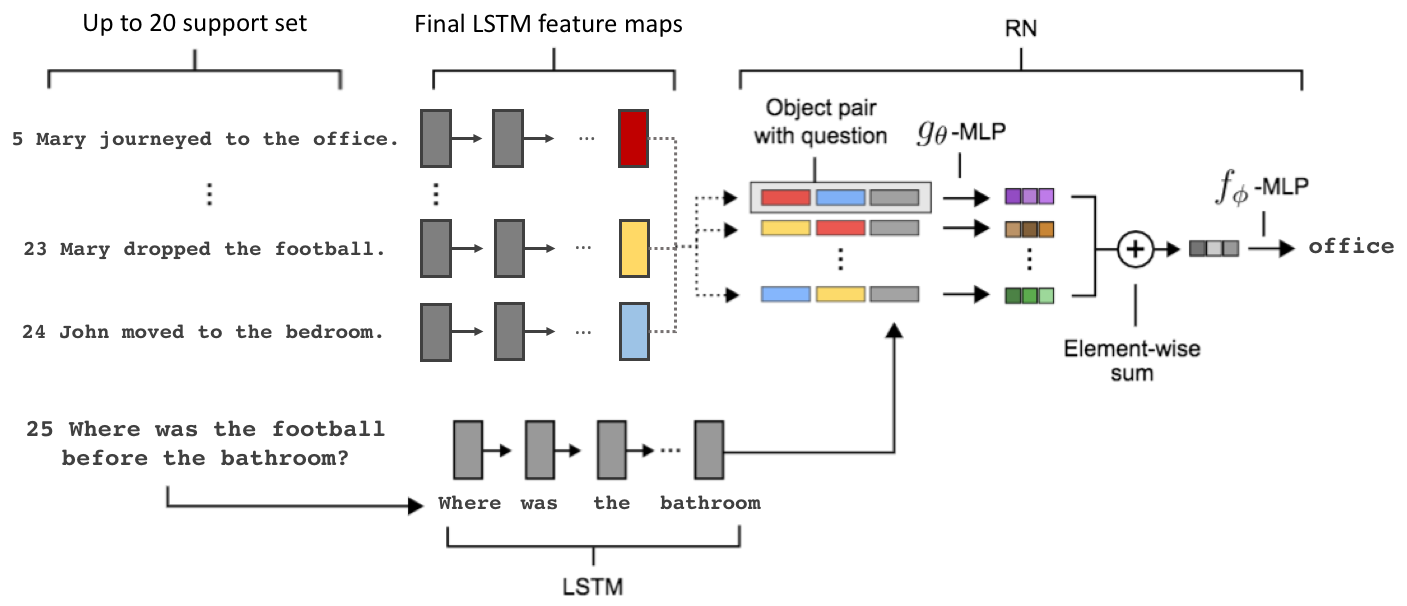
\includegraphics[scale=0.3]{relation_network_babi.png}
%  \fbox{\rule[-.5cm]{0cm}{4cm} \rule[-.5cm]{4cm}{0cm}}
  \caption{Text based QA architecture. Contexts and questions are processed with an LSTM to produce a set of context and question embedding. Objects, colored yellow, red, and blue, are constructed using LSTMs or USE. The RN considers relations across all pairs of objects, conditioned on the question embedding, and integrates all these relations to answer the question. Our alternative approach substities the LSTM with the USE to produce the embeddings.}
\end{figure}

\subsection{bAbI}
The bAbI dataset is a pure text-based question answering (QA) dataset that contains a total of 20 tasks. Each task corresponds to a particular type of reasoning, such as deduction, induction and counting. Every question is associated with a set of supporting facts, which provides the context for the question being asked. An example ``Sandra picked up the football'' and ``Sandra went to the office'' support the question ``Where is the football?'', which we humans can arrive at an easy at the answer ``office''. A task is considered to be successfully passed if it attains an accuracy of 95\% or higher.


\subsection{Two Supporting Fact Task}
Task 2 of the bAbI tasks requires chaining of two or three supporting facts to answer the question. As such, to answer the question ``Where is the football?'', it has to possibly be able to link information from the sentences ``Mary moved to the bathroom'', ``Mary picked up the football there'' and ``Mary went back to the garden'' for it to conclude that the football is at the garden. This tasks makes it challenging for the neural network as it requires some form of memory for it to be able to link previously acquired knowledge to answer the question. 

The RN succeeded on the basic induction task, which proved difficult for Sparse DNC, Differentiable Neural Computer (DNC) \cite{Graves2016} and Sparse DNC \cite{Rae2016}. However, it missed the $95\%$ mark for the ``two supporting fact'' and ``three supporting fact'' tasks, which architectures with memory like Memory Networks \cite{Weston2015a}, DNC and sparse DNC excelled. Thus we focused on task 2 for our project, to investigate if a better representation, in a form the USE obtained from multi-task learning, fare better than unsupervised representations.


%End-to-End Memory Networks \cite{Sukhbaatar2015}


\section{Model}
\begin{enumerate}
\item Overview of the original RN model, comment on the strength and weaknesses
\item Modifications to the RN model that will help improve the accuracy of the task. Motivations for the modifications.
\item (Optional) A paragraph on USE?

\item How long we take to train our model and the train/test accuracy, loss values etc. Use original RN paper as a guideline of what numbers to show.
\end{enumerate}

\subsection{Relation Network}


%For the bAbI suite of tasks the natural language inputs must be transformed into a set of objects. This is a distinctly different requirement from visual QA, where objects were defined as spatially distinct regions in convolved feature maps. So, we first identified up to 20 sentences in the support set that were immediately prior to the probe question. Then, we tagged these sentences with labels indicating their relative position in the support set, and processed each sentence word-by-word with an LSTM (with the same LSTM acting on each sentence independently).
%

The RN is a neural network module which is designed to do relational reasoning. It is a composite function whose form is given by:
\begin{align}
RN(O) = f_\phi\left(\sum_{i,j}g_\theta(o_i,o_j,q)\right)\label{eq:RNform}
\end{align}
where the input is a set of ``objects'' $O=\{o_1,\ldots,o_n\}$, $o_i \in \mathbb{R}^m$ is the $i^{\text{th}}$ object, and $f_\phi$ and $g_\theta$ are function with learnable parameters $\phi$ and $\theta$ respectively. $f_\phi$ and $g_\theta$ are mulit-layer perceptrons (MLP), where $g_\theta$ learns the relation between any two given objects and $f_\phi$ maps the relations to one of the many possible answers. In the next part, we will discuss how using different embeddings lead to different implementations of our model.


\begin{figure}[h]
  \centering
  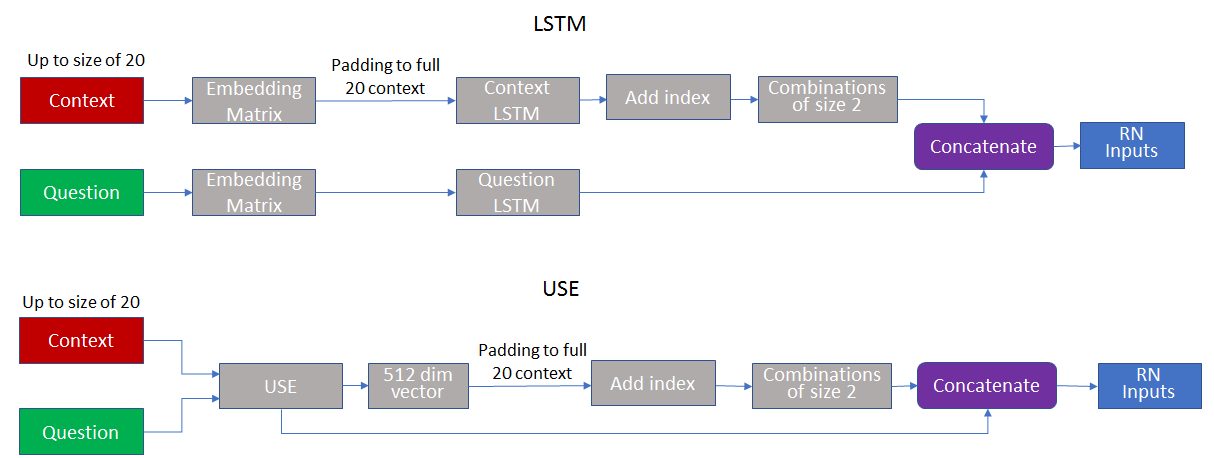
\includegraphics[scale=0.70]{lstmuse.png}
%  \fbox{\rule[-.5cm]{0cm}{4cm} \rule[-.5cm]{4cm}{0cm}}
  \caption{Embedding Pipelines. Padding are done at different stages of the pipline for the different embeddings in which padding is done first for the LSTM, whereas padding is done after passing through the USE. }
\end{figure}


\subsubsection{LSTM Embeddings}

The bAbI suite of tasks requires transformation of the natural language inputs into a set of objects. In the original RN paper, to provide the prior knowledge for the RN to base on, 20 sentences in the support set that were prior to the question of interest were used as the context for answering the question, and each sentence was processed word-by-word with an 32 unit LSTM to obtain a sentence embedding, after which it is tagged with labels to indicate their relative position in the support set to obtain the objects that are the inputs to our RN. A separate LSTM with 32 units was used to process the question. Lastly, the softmax output was optimized with a cross-entropy loss function using the Adamn optimizer with a learning rate of $2e^{-4}$.

From (\ref{eq:RNform}) we see that for a context of size $k$, there are $k(k-1)/2$ unique pairings of the objects. In its implementation, for questions with context sizes that are smaller than 20, we pad it with zeros such that we have a full context size of 20, then let the LSTM process the words to get the context embeddings. The labels that tagged the relative position in the support set, which are just one-hot vectors indicating the position of the sentence in the support set, are then concatenated to the embeddings. Lastly, for each given question embedding, it is concatenated to all possible combination of size 2 to obtain the inputs to the RN, which has dimensions $(190, 136)$, the first value reflecting the number of possible combinations and the other the sum of the dimension of the objects and question embeddings.




\subsubsection{USE Embeddings}

For the USE embeddings, we followed the original RN paper of using up to 20 sentences in the support set as the prior for answering the question. The string form of the raw context and question sentences are fed into the USE which outputs a 512 dimensional vector sentence embedding for each sentence. As such we see that the USE embeddings gives the contexts and questions a much richer representation as compared to the LSTM embeddings.

One main difference from the LSTM embedding approach is that we do not pad the context to the full size of 20 before passing through the USE, compared to padding the context to 20 sentences before letting the LSTM process the words. We note that to do something similar in the USE context, we have to pad the sentences to the same length with a special character, for example ``null''. Instead we keep the sentence length as it is, pass it through the USE to obtain the sentence embeddings and for context with size less than 20, pad it sufficiently with zeros we get 20 contexts. The addition of the one-hot vector labels, we only concatenate the one-hot vectors for those non-trivial contexts, for those padded contexts, the labels are just zero vectors of dimension 20. From experiments, if we were to label the trivial contexts with the one-hot vectors, it gives a very poor performance. As the dimensions of the representation of each sentence for both context and questions is increased from 32 to 512, our inputs to the RN has dimensions $(190,1536)$. 



%For the bAbI task, each of the 20 sentences in the support set was processed through a 32 unit LSTM to produce an object. For the RN, gθ was a four-layer MLP consisting of 256 units per layer. For fφ, we used a three-layer MLP consisting of 256, 512, and 159 units, where the final layer was a linear layer that produced logits for a softmax over the answer vocabulary. A separate LSTM with 32 units was used to process the question. The softmax output was optimized with a cross-entropy loss function using the Adam optimizer with a learning rate of 2e−4.





\subsection{Embeddings}
\textbf{(Short paragraph on embeddings,bert,  Elmo, glove, etc.)}

There are various ways to embed words, from common unsupervised models like word2vec \cite{word2vec} and GloVe \cite{pennington2014glove}. Early this year we have ELMo \cite{N18-1202}, which improved the state of the art embeddings. ELMo differs from other unsupervised embeddings by having their inputs to be characters instead of words, allowing them to take advantage of sub-word units to compute meaningful representations even for out-of-vocabulary words. We shall now discuss the two different embeddings we have used in our experiments whose efficacy we are investigating.

%There has been interesting developments in word embeddings





\subsubsection{LSTM}
For the LSTM embeddings, a randomly initialized word embedding matrix is used to assign each word to a vector representation, which is then passed through a 32 unit LSTM

hashing on the word level, the lstm to obtain an embedding on the sentence level.

\subsubsection{Universal Sentence Encoder}
paper, tensorflow blog

\section{Results}


We have made several comparison between different types of embeddings, different sample sizes, different types of inputs to feed to the RN module and different modifications to the RN module with our implementation of USE embeddings. We compared the accuracy of the test set for different modifications to the RN module and compared the accuracy of the validation set for the rest of the comparisons.

 

For the experiments, all models were run with batch size of 64, with 200 epochs and validation set was taken from the last 10\% of the training set. For the original RN module, $f_\phi \left(\sum_{i,j} g_\theta (o_i,o_j,q)\right)$, $g_\theta$ is a four-layer MLP 256 unites per layer and $f_\phi$ is a three-layer MLP consisting of 256, 512 and 6 units, where the final softmax output was optimized with a cross-entropy loss function using the Adam optimizer with a learning rate of $2e^{-4}$. All models are run on original RN module except for the different modifications to the RN module. The results and weights used are all based on the epoch that gave the best validation accuracy.

 

 

\subsection{Comparison between Different Embeddings}

 

 

We have made comparisons between the two different embeddings of the sentences of the contexts, questions and answers from all data from the training set of Task 2:

 

\begin{itemize}

\item Model LSTM: Use LSTM to embed the sentences of the contexts, questions and answers, and then to pass to the RN module

\item Model USE: Use USE to embed the sentences of the contexts, questions and answers, and then to pass to the RN module

\end{itemize}

 

\begin{center}

\begin{tabular}{|r|r|r|}

 

\hline

\textbf{Model}&\textbf{Training Accuracy ($\%$)}&\textbf{Training Accuracy ($\%$)}\\

\hline

LSTM & &\\

\hline

USE & & \\

\hline

 

\end{tabular}

\end{center}

 

From the results, we can see that based on training solely on the training set of Task 2, using USE embedding provides a much better representation than LSTM embedding in training our RN module. Thus, we will be running the rest of the models with USE embedding.

 

 

\subsection{Comparison between Different Sample Sizes}

 

 

We ran the original model and compared between 2 different sample sizes of the training set:

 

\begin{itemize}

\item  First 1000 contexts of the training set

\item Full 9995 contexts of the training set

\end{itemize}

 

\begin{center}

\begin{tabular}{|r|r|r|}

 

\hline

\textbf{Model}&\textbf{Training Accuracy ($\%$)}&\textbf{Training Accuracy ($\%$)}\\

\hline

First 1000 & 96.2 & 35.0\\

\hline

Full 9995 & 100 & 87.1\\

\hline

 

\end{tabular}

\end{center}

 

Based on the validation accuracy, we can see that it is necessary to include all data in the training set for training of the models. Thus, we will be running the rest of the models based on the full 9995 contexts.

 

 

\subsection{Comparison between Different Modification of the RN Module}

 

For LSTM embedding, each sentence and question had been embedded to a 32-unit object, with sentences from the contexts and questions being processed through separate LSTMs. For each question embedding, it is paired with a combination of 2 sentence embeddings from up to 20 prior sentences, with indexes. Batches of 190 (20 sentences choose 2) combinations of dimension 136 vectors (32-unit sentence $i$ embedding + one hot 20-dimension vector for index of sentence $i$ + 32-unit sentence $j$ embedding + one hot 20-dimension vector for index of sentence $j$ + 32-unit question embedding) with batch size of 64 were passed through the RN module.

 

On the other hand, each sentence and question had been embedded to a 512-unit object with the pre-trained USE. As a result, instead of having 190 combinations of dimension 136 vectors with batch size of 64 being passed through the RN module, we would have combinations of dimension 1576 (512-unit sentence $i$ embedding + one hot 20-dimension vector for index of sentence $i$ + 512-unit sentence $j$ embedding + one hot 20-dimension vector for index of sentence $j$ + 512-unit question embedding). From this we can see that there is an increase in the dimension of each input, and hence, the complexity of each input before passing through the RN module. Thus, we believed by increasing the number of layers or/and number of neurons in each layer would improve the accuracy of the test set as the RN module would have more components to learn from.

 

We compared between different modifications of the RN model and checked for the accuracy of the test set:

 

\begin{itemize}

\item Model ori: Original RN module $(g: [256 \times 4], f: [256,512,6])$

\item Model g6: Increase number of layers of g from 4 to 6 $(g: [256 \times 6], f: [256,512,6])$

\item Model g8: Increase number of layers of g from 4 to 8 $(g: [256 \times 8], f: [256,512,6])$

\item Model 512: Increase number of neurons in each layer of g from 256 to 512 $(g: [512 \times 4], f: [256,512,6])$

\item Model 512f512: Increase number of neurons in each layer of g from 256 to 512 and first layer of f from 256 to 512 $(g: [512 \times 4], f: [512,512,6])$

\item Model g6x512: Increase number of layers of g from 4 to 6 and increase number of neurons in each layer of g from 256 to 512 $(g: [512 \times 6], f: [256,512,6])$

\item Model g6x512f512: Increase number of layers of g from 4 to 6, increase number of neurons in each layer of g from 256 to 512 and first layer of f from 256 to 512 $(g: [512 \times 6], f: [512,512,6])$

\item Model double: Increase number of layers of g from 4 to 6 and double the number of neurons in all layers except for the last layer of f $(g: [512 \times 6], f: [512,1024,6])$

\end{itemize}

 

\begin{center}

\begin{tabular}{|l|c|c|c|}

 

\hline

\textbf{Model}&\textbf{Training Accuracy ($\%$)}&\textbf{Training Accuracy ($\%$)}\\

\hline

ori&100&87.1&85.5\\

\hline

g6&100&89.1&88.4\\

\hline

g8&18.4&22.2&20.0\\

\hline

512&100&88.2&85.0\\

\hline

512f512&99.9&87.9&88.3\\

\hline

g6x512&100&87.8&88.5\\

\hline

g6x512f512&99.7&88.3&89.0\\

\hline

double&100&88.2&88.4\\

\hline

 

\end{tabular}

\end{center}

 

Based on the test accuracies of the above models, we can see that increasing the number of layers of g function from 4 to 6 increased the test accuracy but drastically decreased the accuracy when it was increased to 8 layers. There is also improvement in the test accuracy when the number of neurons for each layer of g function from 256 to 512. The above table shows that the best model for our USE implementation is Model g6x512f512, which is to increase both the number of layers from 4 to 6 and the number of neurons from 256 to 512 for each layer of the g function, together with an increase of number of neurons from 256 to 512 for the first layer of the f function.




\section{Discussion and Conclusions}




\bibliographystyle{abbrvnat}
\bibliography{bib}


%%%%%%%%%%%%%%%%%%%%
%%%%%Template Below%%%%%%%
%%%%%%%%%%%%%%%%%%%%

%\newpage
%
%\section{Submission of papers to NIPS 2018}
%
%NIPS requires electronic submissions.  The electronic submission site
%is
%\begin{center}
%  \url{https://cmt.research.microsoft.com/NIPS2018/}
%\end{center}
%
%Please read the instructions below carefully and follow them faithfully.
%
%\subsection{Style}
%
%Papers to be submitted to NIPS 2018 must be prepared according to the
%instructions presented here. Papers may only be up to eight pages
%long, including figures. Additional pages \emph{containing only
%  acknowledgments and/or cited references} are allowed. Papers that
%exceed eight pages of content (ignoring references) will not be
%reviewed, or in any other way considered for presentation at the
%conference.
%
%The margins in 2018 are the same as since 2007, which allow for
%$\sim$$15\%$ more words in the paper compared to earlier years.
%
%Authors are required to use the NIPS \LaTeX{} style files obtainable
%at the NIPS website as indicated below. Please make sure you use the
%current files and not previous versions. Tweaking the style files may
%be grounds for rejection.
%
%\subsection{Retrieval of style files}
%
%The style files for NIPS and other conference information are
%available on the World Wide Web at
%\begin{center}
%  \url{http://www.nips.cc/}
%\end{center}
%The file \verb+nips_2018.pdf+ contains these instructions and
%illustrates the various formatting requirements your NIPS paper must
%satisfy.
%
%The only supported style file for NIPS 2018 is \verb+nips_2018.sty+,
%rewritten for \LaTeXe{}.  \textbf{Previous style files for \LaTeX{}
%  2.09, Microsoft Word, and RTF are no longer supported!}
%
%The \LaTeX{} style file contains three optional arguments: \verb+final+,
%which creates a camera-ready copy, \verb+preprint+, which creates a
%preprint for submission to, e.g., arXiv, and \verb+nonatbib+, which will
%not load the \verb+natbib+ package for you in case of package clash.
%
%\paragraph{New preprint option for 2018}
%If you wish to post a preprint of your work online, e.g., on arXiv,
%using the NIPS style, please use the \verb+preprint+ option. This will
%create a nonanonymized version of your work with the text
%``Preprint. Work in progress.''  in the footer. This version may be
%distributed as you see fit. Please \textbf{do not} use the
%\verb+final+ option, which should \textbf{only} be used for papers
%accepted to NIPS.
%
%At submission time, please omit the \verb+final+ and \verb+preprint+
%options. This will anonymize your submission and add line numbers to aid
%review. Please do \emph{not} refer to these line numbers in your paper
%as they will be removed during generation of camera-ready copies.
%
%The file \verb+nips_2018.tex+ may be used as a ``shell'' for writing
%your paper. All you have to do is replace the author, title, abstract,
%and text of the paper with your own.
%
%The formatting instructions contained in these style files are
%summarized in Sections \ref{gen_inst}, \ref{headings}, and
%\ref{others} below.
%
%\section{General formatting instructions}
%\label{gen_inst}
%
%The text must be confined within a rectangle 5.5~inches (33~picas)
%wide and 9~inches (54~picas) long. The left margin is 1.5~inch
%(9~picas).  Use 10~point type with a vertical spacing (leading) of
%11~points.  Times New Roman is the preferred typeface throughout, and
%will be selected for you by default.  Paragraphs are separated by
%\nicefrac{1}{2}~line space (5.5 points), with no indentation.
%
%The paper title should be 17~point, initial caps/lower case, bold,
%centered between two horizontal rules. The top rule should be 4~points
%thick and the bottom rule should be 1~point thick. Allow
%\nicefrac{1}{4}~inch space above and below the title to rules. All
%pages should start at 1~inch (6~picas) from the top of the page.
%
%For the final version, authors' names are set in boldface, and each
%name is centered above the corresponding address. The lead author's
%name is to be listed first (left-most), and the co-authors' names (if
%different address) are set to follow. If there is only one co-author,
%list both author and co-author side by side.
%
%Please pay special attention to the instructions in Section \ref{others}
%regarding figures, tables, acknowledgments, and references.
%
%
%\section{Headings: first level}
%\label{headings}
%
%All headings should be lower case (except for first word and proper
%nouns), flush left, and bold.
%
%First-level headings should be in 12-point type.
%
%\subsection{Headings: second level}
%
%Second-level headings should be in 10-point type.
%
%\subsubsection{Headings: third level}
%
%Third-level headings should be in 10-point type.
%
%\paragraph{Paragraphs}
%
%There is also a \verb+\paragraph+ command available, which sets the
%heading in bold, flush left, and inline with the text, with the
%heading followed by 1\,em of space.
%
%\section{Citations, figures, tables, references}
%\label{others}
%
%These instructions apply to everyone.
%
%\subsection{Citations within the text}
%
%The \verb+natbib+ package will be loaded for you by default.
%Citations may be author/year or numeric, as long as you maintain
%internal consistency.  As to the format of the references themselves,
%any style is acceptable as long as it is used consistently.
%
%The documentation for \verb+natbib+ may be found at
%\begin{center}
%  \url{http://mirrors.ctan.org/macros/latex/contrib/natbib/natnotes.pdf}
%\end{center}
%Of note is the command \verb+\citet+, which produces citations
%appropriate for use in inline text.  For example,
%\begin{verbatim}
%   \citet{hasselmo} investigated\dots
%\end{verbatim}
%produces
%\begin{quote}
%  Hasselmo, et al.\ (1995) investigated\dots
%\end{quote}
%
%If you wish to load the \verb+natbib+ package with options, you may
%add the following before loading the \verb+nips_2018+ package:
%\begin{verbatim}
%   \PassOptionsToPackage{options}{natbib}
%\end{verbatim}
%
%If \verb+natbib+ clashes with another package you load, you can add
%the optional argument \verb+nonatbib+ when loading the style file:
%\begin{verbatim}
%   \usepackage[nonatbib]{nips_2018}
%\end{verbatim}
%
%As submission is double blind, refer to your own published work in the
%third person. That is, use ``In the previous work of Jones et
%al.\ [4],'' not ``In our previous work [4].'' If you cite your other
%papers that are not widely available (e.g., a journal paper under
%review), use anonymous author names in the citation, e.g., an author
%of the form ``A.\ Anonymous.''
%
%\subsection{Footnotes}
%
%Footnotes should be used sparingly.  If you do require a footnote,
%indicate footnotes with a number\footnote{Sample of the first
%  footnote.} in the text. Place the footnotes at the bottom of the
%page on which they appear.  Precede the footnote with a horizontal
%rule of 2~inches (12~picas).
%
%Note that footnotes are properly typeset \emph{after} punctuation
%marks.\footnote{As in this example.}
%
%\subsection{Figures}
%
%\begin{figure}
%  \centering
%  \fbox{\rule[-.5cm]{0cm}{4cm} \rule[-.5cm]{4cm}{0cm}}
%  \caption{Sample figure caption.}
%\end{figure}
%
%All artwork must be neat, clean, and legible. Lines should be dark
%enough for purposes of reproduction. The figure number and caption
%always appear after the figure. Place one line space before the figure
%caption and one line space after the figure. The figure caption should
%be lower case (except for first word and proper nouns); figures are
%numbered consecutively.
%
%You may use color figures.  However, it is best for the figure
%captions and the paper body to be legible if the paper is printed in
%either black/white or in color.
%
%\subsection{Tables}
%
%All tables must be centered, neat, clean and legible.  The table
%number and title always appear before the table.  See
%Table~\ref{sample-table}.
%
%Place one line space before the table title, one line space after the
%table title, and one line space after the table. The table title must
%be lower case (except for first word and proper nouns); tables are
%numbered consecutively.
%
%Note that publication-quality tables \emph{do not contain vertical
%  rules.} We strongly suggest the use of the \verb+booktabs+ package,
%which allows for typesetting high-quality, professional tables:
%\begin{center}
%  \url{https://www.ctan.org/pkg/booktabs}
%\end{center}
%This package was used to typeset Table~\ref{sample-table}.
%
%\begin{table}
%  \caption{Sample table title}
%  \label{sample-table}
%  \centering
%  \begin{tabular}{lll}
%    \toprule
%    \multicolumn{2}{c}{Part}                   \\
%    \cmidrule(r){1-2}
%    Name     & Description     & Size ($\mu$m) \\
%    \midrule
%    Dendrite & Input terminal  & $\sim$100     \\
%    Axon     & Output terminal & $\sim$10      \\
%    Soma     & Cell body       & up to $10^6$  \\
%    \bottomrule
%  \end{tabular}
%\end{table}
%
%\section{Final instructions}
%
%Do not change any aspects of the formatting parameters in the style
%files.  In particular, do not modify the width or length of the
%rectangle the text should fit into, and do not change font sizes
%(except perhaps in the \textbf{References} section; see below). Please
%note that pages should be numbered.
%
%\section{Preparing PDF files}
%
%Please prepare submission files with paper size ``US Letter,'' and
%not, for example, ``A4.''
%
%Fonts were the main cause of problems in the past years. Your PDF file
%must only contain Type 1 or Embedded TrueType fonts. Here are a few
%instructions to achieve this.
%
%\begin{itemize}
%
%\item You should directly generate PDF files using \verb+pdflatex+.
%
%\item You can check which fonts a PDF files uses.  In Acrobat Reader,
%  select the menu Files$>$Document Properties$>$Fonts and select Show
%  All Fonts. You can also use the program \verb+pdffonts+ which comes
%  with \verb+xpdf+ and is available out-of-the-box on most Linux
%  machines.
%
%\item The IEEE has recommendations for generating PDF files whose
%  fonts are also acceptable for NIPS. Please see
%  \url{http://www.emfield.org/icuwb2010/downloads/IEEE-PDF-SpecV32.pdf}
%
%\item \verb+xfig+ "patterned" shapes are implemented with bitmap
%  fonts.  Use "solid" shapes instead.
%
%\item The \verb+\bbold+ package almost always uses bitmap fonts.  You
%  should use the equivalent AMS Fonts:
%\begin{verbatim}
%   \usepackage{amsfonts}
%\end{verbatim}
%followed by, e.g., \verb+\mathbb{R}+, \verb+\mathbb{N}+, or
%\verb+\mathbb{C}+ for $\mathbb{R}$, $\mathbb{N}$ or $\mathbb{C}$.  You
%can also use the following workaround for reals, natural and complex:
%\begin{verbatim}
%   \newcommand{\RR}{I\!\!R} %real numbers
%   \newcommand{\Nat}{I\!\!N} %natural numbers
%   \newcommand{\CC}{I\!\!\!\!C} %complex numbers
%\end{verbatim}
%Note that \verb+amsfonts+ is automatically loaded by the
%\verb+amssymb+ package.
%
%\end{itemize}
%
%If your file contains type 3 fonts or non embedded TrueType fonts, we
%will ask you to fix it.
%
%\subsection{Margins in \LaTeX{}}
%
%Most of the margin problems come from figures positioned by hand using
%\verb+\special+ or other commands. We suggest using the command
%\verb+\includegraphics+ from the \verb+graphicx+ package. Always
%specify the figure width as a multiple of the line width as in the
%example below:
%\begin{verbatim}
%   \usepackage[pdftex]{graphicx} ...
%   \includegraphics[width=0.8\linewidth]{myfile.pdf}
%\end{verbatim}
%See Section 4.4 in the graphics bundle documentation
%(\url{http://mirrors.ctan.org/macros/latex/required/graphics/grfguide.pdf})
%
%A number of width problems arise when \LaTeX{} cannot properly
%hyphenate a line. Please give LaTeX hyphenation hints using the
%\verb+\-+ command when necessary.
%
%\subsubsection*{Acknowledgments}
%
%Use unnumbered third level headings for the acknowledgments. All
%acknowledgments go at the end of the paper. Do not include
%acknowledgments in the anonymized submission, only in the final paper.
%
%\section*{References}
%
%
%
%
%References follow the acknowledgments. Use unnumbered first-level
%heading for the references. Any choice of citation style is acceptable
%as long as you are consistent. It is permissible to reduce the font
%size to \verb+small+ (9 point) when listing the references. {\bf
%  Remember that you can use more than eight pages as long as the
%  additional pages contain \emph{only} cited references.}
%\medskip
%
%\small
%
%[1] Alexander, J.A.\ \& Mozer, M.C.\ (1995) Template-based algorithms
%for connectionist rule extraction. In G.\ Tesauro, D.S.\ Touretzky and
%T.K.\ Leen (eds.), {\it Advances in Neural Information Processing
%  Systems 7}, pp.\ 609--616. Cambridge, MA: MIT Press.
%
%[2] Bower, J.M.\ \& Beeman, D.\ (1995) {\it The Book of GENESIS:
%  Exploring Realistic Neural Models with the GEneral NEural SImulation
%  System.}  New York: TELOS/Springer--Verlag.
%
%[3] Hasselmo, M.E., Schnell, E.\ \& Barkai, E.\ (1995) Dynamics of
%learning and recall at excitatory recurrent synapses and cholinergic
%modulation in rat hippocampal region CA3. {\it Journal of
%  Neuroscience} {\bf 15}(7):5249-5262.

\end{document}
